\documentclass{article}
\usepackage[a4paper, total={7in, 9in}]{geometry}
\usepackage{helvet} % required to set arial font
\usepackage[backend=biber,style=numeric,sorting=ynt]{biblatex}
\usepackage{graphicx} % required for the figure
\usepackage[labelformat=empty]{caption}  % required to remove the "Figure 1." from the figure caption


\renewcommand{\familydefault}{\sfdefault} % set arial font
\addbibresource{bibliography.bib}

\title{\titlepartone \newline \titleparttwo}
\author{Directed by Ebbo Demant \\
    \small{Translated from the original German by Jack Borer}
}
\date{} % remove data using this empty command

\newcommand{\I}{Interviewer}
\newcommand{\N}{Narrator}
\newcommand{\OK}{Oswald Kaduk}
\newcommand{\JE}{Josef Erber}
\newcommand{\JK}{Josef Klehr}

\newcommand{\dialogueentry}[4]{
    \begin{center}
    \begin{tabular}{p{1in} p{3.5in} p{1.5in}} 
        #2 \newline \textit{#1} & #3 & \small{#4} 
    \end{tabular}
    \end{center}
}

\newcommand{\seenote}[1]{\textbf{#1}}

\newcommand{\onelinebreak}{\newline}
\newcommand{\twolinebreak}{\newline \newline}

\newcommand{\titlepartone}{Three German Murderers}
\newcommand{\titleparttwo}{A Record of the Banality of Evil}


\begin{document}

\maketitle

\section*{Foreword to the Translation}
\begin{figure}[htp]
    \centering
    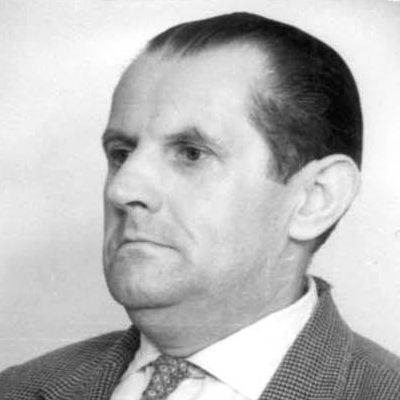
\includegraphics[width=0.3\textwidth]{headshots/ok200by200.png}\hfill
    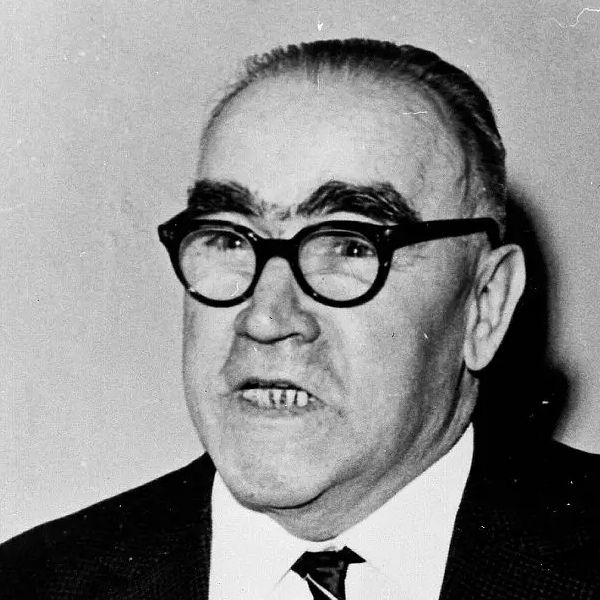
\includegraphics[width=0.3\textwidth]{headshots/je200by200.png}\hfill
    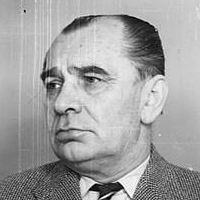
\includegraphics[width=0.3\textwidth]{headshots/jk200by200.png}
    \caption{Three German murderers; \OK, \JE \space and \JK.}
\end{figure}

The Frankfurt Auschwitz trials were a series of criminal trials held in the 1960s to prosecute those directly responsible for the physical horrors of the Auschwitz-Birkenau concentration and extermination camp. Three of those convicted during this process and sentenced to life in prison were Oswald Kaduk, Josef Erber and Josef Klehr. Men who were convicted for their extraordinary brutality and willingness to serve as active executors of Germany's policy to eradicate European Jewry.

In 1978 the three men, while serving life sentences, were interviewed by director Ebbo Demant about their role in the camp and their reflections on their actions. A transcript of these interviews was released in a 1979 book titled \textit{"Straight from the ramp, gone..." Kaduk, Erber Klehr: Three perpetrators go on record} (original German title, \textit{"Direkt von der Rampe weg..." Kaduk, Erber, Klehr: Drei Täter geben zu Protokoll})\cite{DirektVonDerRampeWeg}. However the film, the only filmed interviews with Frankfurt Auschwitz trial perpetrators, went unused. In 1999 Ebbo Demant revisited the material and released a 44 minute film titled \textit{\titlepartone \space \titleparttwo} (original German title, \textit{Drei deutsche Mörder. Aufzeichnungen über die Banalität des Bösen})\cite{DreiDeutscheMörder}. 

This document is an English translation of the interviews found in this film, intended to make the material more accessible. While the words of a perpetrator should not be considered the words of a passive truthful observer, the following interviews provide a stunning look in the machinery of the Holocaust; from men who openly admit to beating prisoners, injecting sick powerless people with phenol and tallying and recording the number of those selected on the ramp to live and those selected for extermination. This film serves as a reminder that we must never forget.

\newpage

\dialogueentry{00:01}{\N}{Oswald Kaduk, born 1906, high school graduate, butcher by trade. 1939 enlisted in the SS. Since 1941 in Auschwitz, Rapportführer\seenote{*}. 1959 arrested, 1965 sentenced to life in prison for ten murders and at least 1000 communal murders \seenote{**}.). 1989 released. 1997 passed away as a pensioner.
\twolinebreak
Josef Erber, born 1897,  high school graduate, textile worker by trade. 1939 enlisted in the SS. Since 1940 in Auschwitz, Oberscharführer\seenote{***}. 1962 arrested. 1966 sentenced to life in prison for 70 communal murders. 1986 released. 1987 passed away as a pensioner.
\twolinebreak
Josef Klehr. Born 1904,  high school graduate, woodworker by trade, practicing nurse. 1932 enlisted in the SS. Since 1941 in Auschwitz, medic. 1960 arrested. 1965 sentenced to life in prison for 475 murders and as an accessory to communal murder in 1,980 cases. 1988 released and passed away in the same year as a pensioner.}{
\seenote{*}A Rapportführer (literally "report leader") was a non-commissioned officer responsible for supervising multiple camp Blocks.
\onelinebreak
\seenote{**} The phrase "gemeinschaftlichen Mordes" translates directly to "communal murder". This is when murder is committed as part of a group. A more meaningful English translation or equivalent is unclear. 
\onelinebreak
\seenote{***}A Oberscharführer was a non-commissioned officer SS rank equivalent to the US military's sergeant first class.
}

\dialogueentry{01:53}{Caption}{\titlepartone
\twolinebreak
\titleparttwo
\twolinebreak
From Ebbo Demant}{}

\dialogueentry{02:08}{\OK}{Well yeah, there was a street and in front there was a big gate that said "Work sets you free". At that time the street was expanded and improved and the prisoners were distributed to work. 
\twolinebreak 
I didn't have anything to do with it. Was the work hard, absolutely, but not us. My only responsibility was that everything ran smoothly and that the evening roll call was correct. I couldn't do anything about it. Of course today people accuse me of being responsible.}{}

\dialogueentry{02:53}{\I}{During the trial you once described that when you got to Auschwitz you started to drink there.}{}

\dialogueentry{03:02}{\OK}{Yeah, I am open about that. In my entire life I never drank as much alcohol as I did in Auschwitz. They might laugh about that. Sometimes when I went to distribute the block leaders to their posts in the morning, I had already had a drink at 9AM, that's how I was. My boss knew that I was drinking. But it wasn't so obvious that I was staggering around.}{}

\dialogueentry{03:36}{\I}{And why did you drink?}{}

\dialogueentry{03:37}{\OK}{I've already said, it doesn't matter why.}{}

\dialogueentry{03:41}{\JK}{I came in from the front and I could already smell the infection ward. I was able to smell it all the way from the camp gate when the wind came from the right direction. 
\twolinebreak
All the infected were lying there, with open wounds on their legs, others with tuberculosis or typhus or other diseases, it could be anything. Diseases that weren't even known in Germany. The camp doctor couldn't even diagnose typhus when it broke out. A polish prisoner camp doctor made the diagnosis instead.}{}

\dialogueentry{04:39}{\I}{Did the death of these people do anything to you or touch you in any way?}{}

\dialogueentry{04:43}{\JK}{Yeah, you can't get any closer to it than that. When you see that every day, you wake up early and you start to feel sick on the way to your shift. It goes from morning to night and you don't have time to reflect and think about it.}{}

\dialogueentry{04:58}{\JE}{At the start it was slow and there were not that many people because there were no large transports. The transports began in 1942 when the so-called RSHA transports came.}{}

\dialogueentry{05:13}{\I}{What are those?}{}

\dialogueentry{05:14}{\JE}{The transports from the Reichsicherheitshauptamt\seenote{*}  that came from abroad. Those were outright pure Jew transports.}{\seenote{*}"Reich Security Main Office"}

\dialogueentry{05:23}{\I}{And then they were all registered?}{}

\dialogueentry{05:26}{\JE}{No. Only those that went into the camp were registered.}{}

\dialogueentry{05:34}{\I}{And the others that didn't go into the camp?}{}

\dialogueentry{05:36}{\JE}{The others were on the so-called "ramp", in the meantime the ramp at Birkenau which had been expanded and built out was finished\seenote{*}. And when a train came in with a transport the transport commander had to let the people out and line them up for roll call. 
\twolinebreak
At that time I was in the political unit and was there at the intake. When I had service on the ramp I had to confirm to the transport commander the number of people they had brought. And then when the entire transport was counted we gave him a receipt that confirmed the delivery of the transport. And then he and the train's guard personnel had to leave the ramp. And then the doctor started with the selection.}{\seenote{*} He changes his thought halfway through the sentence, making the sentence hard to follow. }

\dialogueentry{07:00}{\I}{What is that?}{}

\dialogueentry{07:01}{\JE}{The sorting. For example young people, those that were capable of working would go to work, and the others had to go to the gas chamber.}{}

\dialogueentry{07:17}{\I}{Straight from the ramp into the gas chamber?}{}

\dialogueentry{07:19}{\JE}{Straight from the ramp, gone. But before that, roll call was taken again. Because Berlin required us to precisely count and record the number of men and women.}{}

\dialogueentry{07:43}{\I}{Were you ever at the ramp for a selection?}{}

\dialogueentry{07:45}{\JK}{No, never.}{}

\dialogueentry{07:47}{\I}{You only heard about it?}{}

\dialogueentry{07:48}{\JK}{I only heard about it. When you are there for four years in Auschwitz you hear things and you see things.}{}

\dialogueentry{07:58}{\I}{But how large was the capacity of the individual transports? Roughly how many people came with each transport onto the ramp?
}{}

\dialogueentry{08:07}{\JE}{It was always different. It could be 200, it could be just a single truck, it could be 2,000.}{}

\dialogueentry{08:21}{\I}{In which year came the most transports?}{}

\dialogueentry{08:26}{\JE}{The most transports came in 1944 because that was when Hungary happened.}{}

\dialogueentry{08:42}{\I}{What portion of the people had to work, and what portion were sent directly to the gas chamber?}{}

\dialogueentry{08:53}{\JE}{You can calculate as a percentage that 30\% went to work.}{}

\dialogueentry{09:01}{\I}{And 70\% to the gas chamber?}{}

\dialogueentry{09:04}{\JE}{And 70\% gone.}{}

\dialogueentry{09:06}{\I}{Nowadays there are lots of people that say Auschwitz was a lie and that no one was gassed there.}{}

\dialogueentry{09:11}{\OK}{How should I say it. People that say things like that I don't consider normal. What was it then? Let's be honest. There are some people who only want to dispute it. There is nothing to dispute, what happened happened.}{}

\dialogueentry{09:29}{\JE}{It was four crematoriums. I'm talking about Birkenau. A small one was in Auschwitz but the oven was demolished in 1943 and it wasn't in operation anymore. But for example, outside there was crematorium one and two along the ramp extension. On the left side number one and on the right side number two. Those were the big ones, they had a capacity of 3,000 people.}{}

\dialogueentry{10:17}{\I}{When a transport arrived in Birkenau, how would you describe the mood on the ramp? The people after all were trapped for days in cramped train cars but for you that was a routine. There must have been an exceptional situation between the people there. Can you please describe that?}{}

\dialogueentry{10:49}{\JE}{It completely depended on where they came from. I mean for example we got transports from France where they arrived in Pullman cars. Then we got transports that came in D-Zug\seenote{*} cars. Then we got transports that came in normal regional trains. Of course the most transports came in cattle cars. 
\twolinebreak
And when the transport arrived, for example, at Birkenau outside on the ramp, first the locomotive was decoupled and drove away. The guards were already there and had set up a chain of guard posts. Then the political section and the camp doctor who was on call that day was there. And the people from the material department were there because of the clothes and all the stuff that people brought with them. 
\twolinebreak
And when the transport arrived and everything was setup, the transport commander that brought the transport had to open the doors and organize the people in five rows so that they could be counted by us. In Birkenau right around the ramp there was a block leader barracks that had two rooms. That is where the transport commander would bring the receipt and confirm the number, and then I would give him the ticket. 
\twolinebreak
When they were gone, the train escort squad, the people were lined up in rows that had to walk past the doctor. And there the selection happened for those who had to go into the camp and those who had to go into the gas. And them the people were reorganized again, the women that went into the women's camp and the men that had to go to the men's camp and the third group, the people that had to go into the gas. 
\twolinebreak
And then, when that was done, came a commando, a so-called "clean-up squad", that had to clean out the train cars of the baggage. We had told them that they could leave their things inside. Only by Schutzhäftlingen\seenote{**} did everything have to be recorded, the amounts of money and everything else. But those were RHSA transports and there was nothing to record. Everything was already taken from them by the time they got there. 
\twolinebreak
The people, there was often a little bit of scuffling here and there because some people wanted to stay together, but never to a point where we had to use violence or anything like that. The saying went, "On the ramp everything as calm as possible, so that everything runs smoothly".}{\seenote{*}A "D-Zug" was a class of high speed, long-distance trains commonly used for civilian train travel. 
\onelinebreak
\seenote{**}The term "Schutzhäftlingen" is used to describe political prisoners in the concentration camp system and others that were serving prison sentences instead of those who were exterminated immediately.}

\dialogueentry{15:59}{\I}{There were also selections in the main camp, the so-called "camp selections"}{}

\dialogueentry{16:05}{\OK}{Yep, there were. Mr. Klehr did it with a camp doctor, he always made the decision. We always knew exactly how many sick we had, we had it written down on a card. When there were too many sick he would come and tell the Schutzhaftlagerführer\seenote{*}, "you know what," he would say "I have to do a selection, we have too many people, not enough free beds and not enough supplies." Then they would do a selection that day, a Tuesday or usually a Monday, whenever it was. 
\twolinebreak
Then the prisoner doctors would come collect the prisoner's cards, and then the prisoners would walk by the doctor and medic\seenote{**}. There the doctor would decide if they went to the left or right and would turn the card in the respective direction. Those that were selected went to the right side and those that got to stay went to the left side. And then the groups came back together. The next day the trucks came in the evening, around 17:00 or 18:00, loaded them, and drove them off to Birkenau where they were then registered. 
\twolinebreak
I'm spit balling but for example, 150 or 200 or 220 "please remove them from the infirmary list". And the block leader had to make sure everything was written correctly down in the book, the numbers had to match exactly. The door opened they walked by the guards and then they drove away.}{\seenote{*} A Schutzhaftlagerführer (literally "preventive detention camp leader") was a commissioned SS officer responsible for the operation of the camp. As a Rapportführer \OK would have reported directly to the Schutzhaftlagerführer.
\onelinebreak
\seenote{**} Here is referring to a SS camp doctor and a SS medic.
}

\dialogueentry{18:01}{\I}{Did the prisoners know what was waiting for them?}{}

\dialogueentry{18:03}{\OK}{Yeah, that was clear, they knew. When you've been in the camp so long and then you are sick and you notice that your comrades did not come back. Maybe if they came back then they wouldn't think so. But they knew exactly that that goodbye was the final goodbye. But as sad as it sounds...}{}

\dialogueentry{18:31}{\JK}{Yea, let me start like this. The prisoners that felt sick, they had to report to the Rapportführer on the block. The Rapportführer summarized the list of those that were sick and then gave it to the SS man in the HKB.}{}

\dialogueentry{18:49}{\I}{HKB means Häftlingskrankenbau\seenote{*}?}{\seenote{*}"prisoner's infirmary" or "prisoner's hospital"} 

\dialogueentry{18:50}{\JK}{Häftlingskrankenbau. And in the HKB they came into an extra room and were led one at a time into the treatment room. And the prisoner doctor made the diagnosis and wrote the diagnosis, like I already said, onto the diagnosis card.}{}

\dialogueentry{17:09}{\I}{The prisoner doctor was himself a prisoner?}{}

\dialogueentry{19:13}{\JK}{Yes, he was a prisoner. A prisoner doctor and we also had prisoner nurses, Funktionshäftlinger\seenote{*}. When the prisoner doctor was done, they went back into the main room and had to wait until the camp doctor came. When the camp doctor came I had to accompany him for the visit.}{\seenote{*}"functionary prisoners" were prisoners given administrative roles within the camp. Functionary prisoners tasked with disciplinary roles are often derogatorily referred to as "Kapos".}

\dialogueentry{19:29}{\I}{The camp doctor was an SS doctor?}{}

\dialogueentry{19:31}{\JK}{Yes, that was an SS doctor, SS camp doctor. I had to accompany him to the inspection, and the camp doctor took the diagnosis card, looked what was on there, and without further investigation, just looking at what the prisoner doctor wrote down, decided if the prisoner would go to the infirmary as sick, or recovery for 14 days or three weeks or special treatment.}{}

\dialogueentry{20:02}{\I}{What does special treatment mean?}{}

\dialogueentry{20:04}{\JK}{That was the injections. The death by injection. Special treatment.}{}

\dialogueentry{20:08}{\I}{Can you please describe the special treatment?}{}

\dialogueentry{20:11}{\JK}{Yeah sure, how should I describe it? There were prisoners that were gassed and then there were small groups of prisoners who were killed with injections in the main camp infirmary.}{}

\dialogueentry{20:28}{\I}{How did it happen?}{}

\dialogueentry{20:30}{\JK}{The prisoners were taken from block 28, where the infirmary was, to block 20. In block 20 was an infection section. They came into a room and were then taken out one by one.   In block 20, the first room on the right side, that is where it was carried out. And before the needle was even out, they collapsed in the seat, and two prisoners would come and carry them back into the room across the hall. When everything was over the truck came and took all the corpses to the crematorium.}{}

\dialogueentry{21:17}{\I}{Can you please precisely describe the injection process again?}{}

\dialogueentry{21:22}{\JK}{You know you are killing me right? You're killing me. How should I describe it? With what?}{}

\dialogueentry{21:30}{\I}{How was it when the prisoners came in? Could they feel that they were about to be killed?}{}

\dialogueentry{21:38}{\JK}{I already told you that. The prisoners didn't cry; they didn't defend themselves; they were brought in and sat there on the stool until it was over. Not a word spoken, nothing.}{}

\dialogueentry{21:53}{\I}{And they got the injection directly to the heart?}{}

\dialogueentry{21:55}{\JK}{It was injected directly into the heart muscle. The veins were too deep, it was hard to find them, you had to try three or four times before you found it.}{}

\dialogueentry{22:07}{\OK}{I've seen lots of dead people. Of course, I admit that myself. I saw how they were removed. They were usually taken out around 18:00 with a wagon. There were days when the special tribunal from Katowice or Krakow came and held executions in block 11. It was gruesome. 
\twolinebreak
The door was opened and prisoners walked in with their wagon that they used to remove the bodies. And you can imagine that when they weren't killed with gas, but by gunshot instead, you can imagine what was in there. Blood, with so many, hundreds of dead. And as they drove out with their wagon, the wheels left trails of blood in the dirt behind it. We had it cleaned up, but we couldn't do anything else. I couldn't just say, "Stop, we are done here. What you are doing is a crime".}{}

\dialogueentry{23:30}{\I}{Have you ever thought about the idea that you are yourself guilty?}{}

\dialogueentry{23:35}{\OK}{Yeah sure, I was guilty when I put the uniform on. The SS was a criminal organization.}{}

\dialogueentry{23:53}{\I}{Yes, but what about yourself?}{}

\dialogueentry{23:54}{\OK}{Yeah, I also said that. We were in a war. 35 years after the war and look around the world, what is happening. People are fighting everywhere, resistance fighters are being executed, its a world problem, and its actually gonna get worse. Who knows what's gonna happen, but in a couple years there is going to be a terrible war. I don't want to experience that, I really don't. 
\twolinebreak
Maybe it wasn't right, of course. We were at war and there was death, left and right, but we had bad luck and lost the war.}{}

\dialogueentry{24:37}{\I}{What is a human life worth to you?}{}

\dialogueentry{24:39}{\OK}{Nothing. Nowadays a human life isn't worth anything. }{}

\dialogueentry{24:47}{\I}{And for you personally at that time?}{}

\dialogueentry{24:49}{\OK}{Well at that time to some extent. But today, a drunk driver runs someone over on the highway and keeps on driving without even thinking about it. How are you supposed to consider that Christian? It isn't and I also don't think that is right.}{}

\dialogueentry{25:14}{\I}{At that time did you ever try to understand the individual people and their lives?}{}

\dialogueentry{25:20}{\OK}{Yeah, I used to tell myself hopefully everything will be ok.}{}

\dialogueentry{25:26}{\I}{Were prisoners also killed in the main camp?}{}

\dialogueentry{25:31}{\JE}{Yes, I think that was 1941. But I only heard about that later. At that time I wasn't with the political department yet.}{}

\dialogueentry{25:46}{\I}{What happened there?}{}

\dialogueentry{25:48}{\JE}{In block 11, that was the so-called bunker. In the basement they had made airtight rooms, the first place where anyone was gassed, where people were gassed with Zyklon-B.}{}

\dialogueentry{26:17}{\I}{And did you also see how people were shot on the black wall?}{}

\dialogueentry{26:21}{\JE}{No.}{}

\dialogueentry{26:22}{\I}{Did you hear about it?}{}

\dialogueentry{26:23}{\JE}{I never went there. I knew where the black wall was, but I didn't have anything to do with the executions there because I was at the intake.}{}

\dialogueentry{26:35}{\I}{Did you hear about the shootings?}{}

\dialogueentry{26:37}{\JE}{What was that?}{}

\dialogueentry{26:38}{\I}{Did you hear that people were shot there?}{}

\dialogueentry{26:40}{\JE}{Yes, in 1941 and 1942 almost every week a special tribunal, like they had at that time, came and announced the death sentences there in Auschwitz.}{}

\dialogueentry{27:02}{\OK}{They were selected and then sent to Block 11. They corralled them into Block 11 and it didn't take long for the execution order from Berlin to arrive. The executions should be carried out on Tuesday or whatever day at the roll call. I would be given the order to prepare everything and would confirm with the officer that I would carry out the order. 
\twolinebreak
When there is an order in the camp that there should be five prisoners, then there cannot be seven. Everything has to be counted. One dog after another. When you have the order to do one after another then you have to carry out that order. Distance so and so and there is nothing to think about, nothing to change. My camp commander asked me to do it and I carried out the order. There is nothing to change about it.}{}

\dialogueentry{28:07}{\I}{And when that wasn't...}{}

\dialogueentry{28:08}{\OK}{And every soldier on the front did the same thing. They carried out orders, if they were right or not, it doesn't matter. If you received an order it has to be carried out.
\twolinebreak
Sure that was the front and of course you can say Auschwitz was in the rear, and you can say that Auschwitz was an extermination camp. But if we won the war, the prisoners wouldn't be in the camp today, they would have been released. They would not be in the camp today if we won the war. They wouldn't be there in the camp.}{}

\dialogueentry{28:34}{\I}{They would already all be dead.}{}

\dialogueentry{28:35}{\OK}{Nope. But maybe they would have helped rebuild Germany. That would have been a political question. We already had construction groups with wagons, places where the prisoners could sleep. Everything was already prepared. But everything went wrong, in the end it didn't work out that way in the end. They would not have exterminated them. They would not have exterminated laborers, definitely not. But it turned out differently. Maybe it wasn't meant to be. (\seenote{*})}{\seenote{*} The last 30 seconds of this section from 29:07-29:37 is unintelligible.}

\dialogueentry{29:38}{\I}{But that doesn't need to be  handled with beatings and killings.}{}

\dialogueentry{29:41}{\OK}{How are you supposed to do it? Should I deal with them with silk gloves on? Come on, please. We are talking about normal people that actively decided to do something, and when I said that something is forbidden then it is forbidden. 
\twolinebreak
That is my view on it, that is how I was raised. You take something off the table and it's my property, then they are not allowed to take it, regardless of what it is. People don't believe what I am saying, but what should I do? Sure I know it wasn't right that I beat them, but what was I supposed to do?}{}

\dialogueentry{30:28}{\I}{Were there prisoners that sought death out?}{}

\dialogueentry{30:31}{\JE}{Yeah, there were. Those that jumped directly onto the high voltage fence.}{}

\dialogueentry{30:46}{\OK}{Yes, I admit. When a prisoner wasn't at his work place or had something forbidden, I reported him. He would be led away, and would get sentenced a punishment from the watch leader or camp commander. Either a beating, or three weeks at the casting pits, or two weeks at the sand pits, depending what the commander decided. 
\twolinebreak
Yeah, I know that I have been accused of a lot of things by the prisoners. I told the honorable judge that if that is true, everything that the prisoners accuse me of is true, then I'm nothing. But it isn't anything but vengeance and retribution, it isn't worth anything.}{}

\dialogueentry{31:42}{\I}{But you beat the prisoners?}{}

\dialogueentry{31:44}{\OK}{Yes I beat them, I admit that, but I didn't beat them to death. I beat them often I admit that, given the situation I don't want to say this. But I gave them boxes of sand, we called them spittoons, they were responsible for covering it up with sand and sometimes they would spit in the camp or on the sidewalk \seenote{*}.
\twolinebreak
I would tell them to come over and then ask, "Do you do it like this at home?". They would answer "no", and then I would beat them, one or two blows. If they weren't going fast enough I would give them a hit on the buttocks. It had to be like that, there was no other way to do it. Of course I wasn't well liked, that's obvious.}{\seenote{*} It is unclear to what he refers to here. He might literally mean a spittoon for spitting, or euphemistically chamber pots for human excrement.}

\dialogueentry{32:49}{\I}{You've been called the "terror of the camp".}{}

\dialogueentry{32:50}{\OK}{What does "terror of the camp" even mean? People have accused me of that before, its all baloney. What does "terror" even mean? I wasn't a terror. The others weren't even there at that time, nowadays I'm the terror of Auschwitz.}{}

\dialogueentry{33:16}{\I}{What was done with the corpses?}{}

\dialogueentry{33:22}{\JE}{At the start, the corpses from the gassing were buried. But after some time a bloody liquid started to come out of the ground and the ground became unstable. Then they were dug up and burned.  By that point the crematoriums were ready for that. Four units were brought into operation in 1943}{}

\dialogueentry{34:00}{\I}{And could someone notice from the color of the light or anything else that people were being burnt there?}{}

\dialogueentry{34:08}{\JE}{Yes, first of all, the furnaces where there was always a temperature of 1500 to 1800 degrees\seenote{*}, was like in earlier times when they made porcelain. There was a flame one or two meters shooting out of the chimney. It was just like that and you could smell the scent of burning people all the way to the train station.}{\seenote{*}2732 to 3272 $^{\circ}$F}

\dialogueentry{34:52}{\I}{Does this smell still follow you?}{}

\dialogueentry{34:54}{\JE}{What was that?}{}

\dialogueentry{34:55}{\I}{Does this smell still follow you?}{}

\dialogueentry{34:58}{\JE}{Yes. I mean we couldn't change anything.}{}

\dialogueentry{35:11}{\I}{What was done with the ashes of the corpses?}{}

\dialogueentry{35:14}{\JE}{Part of the ashes were spread in the soil and the rest of the ashes were thrown the rivers.}{}

\dialogueentry{35:37}{\I}{Did you at that time ever personally have any scruple?}{}

\dialogueentry{35:40}{\OK}{No, not even a little bit.}{}

\dialogueentry{35:43}{\JK}{Yeah, very diluted phenol is also used for things like ear injections. But the thing with phenol, like I already said, was started by a former camp commander named Fritzsch.
\twolinebreak
They tested it for the first time in Block 11, that is also where they tested gassing. They tried lots of different things, prisoners told me that the camp doctors tried lots of things. They tried injecting air, gasoline, and everything else before they settled on phenol. They used to use lots of different things, but that was before I showed up, and like I said, I only heard about that from the prisoners.}{}

\dialogueentry{36:45}{\I}{How was it, the prisoners came into the room, and you were standing there with the needle?}{}

\dialogueentry{36:52}{\JK}{I was in the room and the prisoner was led in down the hallway. He couldn't go to the left or right. A prisoner who was my assistant prepared the injection and then I performed the injection.}{}

\dialogueentry{37:09}{\I}{Directly into the heart?}{}

\dialogueentry{37:10}{\JK}{Directly into the heart.}{}

\dialogueentry{37:12}{\I}{Did all prisoners die immediately?}{}

\dialogueentry{37:14}{\JK}{They were dead instantly. Before the needle was even pulled out they were already dead. This death wasn't as terrible as the gassing, that was a terrible death. They came into the gas chamber and the camp doctor gave the order to the SS men on the roof to pour the gas in. Then this noise like the noise from a beehive would emanate from the room "mmmmm... mmmmm... mmmmm" and the sound would get quieter and quieter until there was silence. That was a terrible death, the gas attacked the lungs.}{}

\dialogueentry{38:05}{\I}{But you had to look the people in the face.}{}

\dialogueentry{38:09}{\JK}{Yeah sure, by the injection, what else was I supposed to do? That's what I'll ask you, what should I have done instead?}{}

\dialogueentry{38:16}{\I}{No, you said that the gas chamber was a more gruesome death, but it is at least an anonymous death.}{}

\dialogueentry{38:23}{\JK}{I saw it. The corpses were green and blue when they were removed from the gas chamber, and it lasted longer than the injection. Like I already said, before you even took the needle out they were dead. But by the gassing the noise lasted at least ten minutes, and then got quieter and quieter. That is what I mean when I say that the gassing was more gruesome.
\twolinebreak
The entire thing gruesome, regardless if it was by injection or gassing, but there was a difference and it wasn't as hard. I've thought about this a lot. I observed the prisoners, they never shied away or cried. It was an open secret that when they were led out, it led to death. They knew it. I could never understand then why no prisoner ever cried. I can't understand it. I can only imagine that they were thinking, "Thank God I'm up next." That is the impression I got.}{}

\dialogueentry{39:40}{\I}{There was never anyone that begged or asked for mercy?}{}

\dialogueentry{39:44}{\JK}{No, never! That's what I've thought about. Did someone ever say, "Please Oberscharführer, please let me live."? Never even a peep, not a single word.}{}

\dialogueentry{39:59}{\I}{There are people today that claim that gassing never occurred in Auschwitz. What do you say to that?}{}

\dialogueentry{40:08}{\JE}{I can say the following. I ordered the book \textit{Hexen-Einmal-Eins einer Lüge}\seenote{*}, about the six million dead that people talk about. And among other things, he wrote that there were no death factories and no crematoriums and so on and so forth. I wrote to the publisher, no actually the seller of the book. I asked them for the contact information of the author. After some time they responded and told me that the author is dead, and the publisher is in Upper Franconia. The publisher would be interested if I want to write them. 
\twolinebreak
I wrote them clearly that it was not true, that the crematoriums were really there. The gassing was stopped in October 1944 and the crematoriums were completely destroyed. The iron components were loaded into wagons and were taken to Mauthausen in Austria. I can't understand, because it did happen and how someone today comes to the conclusion that it wasn't real, I just can't understand.}{\seenote{*}A holocaust denial book written by Emil Aretz and published in 1970. The title, \textit{Witches Algebra a Lie}, is a play on words taken from a scene in Johann Wolfgang von Goethe's well known 1808 tragic play titled \textit{Faust: A Tragedy} \cite{HexenEinmalEins}. The title's intent, and that of the book itself, is to call into question the number of Jews murdered in the Holocaust, using widely discredited Holocaust denial talking points \cite{HolocaustReferenzEmilAretz}.}

\dialogueentry{42:12}{\I}{Do you have an explanation for that?}{}

\dialogueentry{42:17}{\JE}{Yes. Either they really don't know the truth or they want to pull the wool over people's eyes. What happened can't be lied away. It actually happened.}{}

\dialogueentry{42:54}{Caption}{\titlepartone \space \titleparttwo
\twolinebreak
From Ebbo Demant
\twolinebreak
Camera Jürgen Bolz
\twolinebreak
Editor Eva Maria Franke
\twolinebreak
Sound Norbert Fischer
\twolinebreak
Editorial Peter Latzel}{}

\newpage

\printbibliography

\end{document}
